% 第 5 章：来自物理的动机
\chapter{来自物理的动机}\label{ch:physics-motivation}
本章旨在介绍镜像对称理论背后的物理动机。我们将简要勾勒从经典物理到超弦理论的发展脉络，并说明 A 模型与 B 模型在超弦理论\index{xianlilun@弦理论|hyperpage}中的来源。关于底层物理的更多细节，可参阅讲义\bookcite{62,251}和专著\bookcite{64,114}。

随后，我们将从范畴论的角度考察物理学，重点放在其代数结构上，并暂且假定路径积分形式等技术问题都能够妥善处理。

\section{路径积分形式}
\takeaway{经典物理用最小作用量原理在构型空间寻找临界点；量子理论则以路径积分把配分函数与可观测量的期望值写成对所有路径的求和，作用量以 $e^{iS/\hbar}$ 加权，$\hbar\to0$ 时只有经典解有贡献。}
\subsection{最小作用量原理}
经典物理的许多方面都可以用最小作用\index{zuoyong@作用|hyperpage}量原理来描述：系统状态的演化方式使某个称为作用量的量达到最小。

例如，设一粒子在流形 $M$ 上运动，其运动可由光滑曲线 $\gamma\colon[a,b]\to M$ 描述。记所有此类路径组成的空间为 $X$。作用量可视为一个函数 $S\colon X\to\mathbb R$。若指定粒子的起点与终点 $x_a,x_b\in M$，则粒子所走的路径应当使作用量在
\[
  X(x_a\to x_b)=\{\gamma\in X\mid \gamma(a)=x_a,\ \gamma(b)=x_b\}
\]
上取最小值。

系统中的每个可观测量都可以看成函数 $F\colon X\to\mathbb R$。例如，时刻 $u\in[a,b]$ 的速度是函数 $v_u\colon X\to\mathbb R$，其定义为 $v_u(\gamma)=\frac{d\gamma}{dt}(u)$。借助最小作用量原理求出解之后，只需将解代入可观测量，就能得到它的取值。所有可观测量共同构成一个代数 $\mathcal O$。

\begin{note}\label{note:classical-physics-observation}
\textbf{观察 5.1.} 经典物理的工作，是在构型空间中寻找临界点，并在这些临界点上计算函数（可观测量）的值。
\end{note}

\subsection{量子理论}
量子力学的主要思想是：粒子并不沿着一条预先指定的路径运动，而是所有可能路径都会以一定的振幅对观测结果作出贡献。在量子力学的路径积分形式\index{lujingjifenxingshitixi@路径积分形式体系|hyperpage}中，我们把 $X$ 看作带测度 $(X,[d\gamma])$ 的可测空间，并在其上积分。一般而言，这一步并不简单；这里我们假定这样的测度存在。量子系统的行为由理论的配分函数\index{peifenhanshu@配分函数|hyperpage}和可观测量的期望值决定，它们定义为
\[
  Z=\int_X e^{iS(\gamma)/\hbar}[d\gamma],\qquad
  \langle F\rangle=\int_X F(\gamma)e^{iS(\gamma)/\hbar}[d\gamma],
\]
其中 $S$ 是经典作用量，$\hbar$ 是普朗克常数。
% [Tutor Note: 原文把 $X$ 直接当作可测空间并写出路径积分，这里省略了两点：其一，Feynman 测度 $[d\gamma]$ 一般不存在 $\sigma$-可加版本，需用 Wick 旋转或格点正则化才能严格定义；其二，物理文献通常把期望值归一化为 $\langle F\rangle=Z^{-1}\int F e^{iS/\hbar}[d\gamma]$，原文未除以 $Z$。]

令普朗克常数 $\hbar$ 趋于 $0$，便能看出量子物理与经典物理之间的联系。若 $S(\gamma)$ 变化很大，$e^{iS(\gamma)/\hbar}$ 就会快速振荡，而相应路径对积分的贡献彼此抵消。在极限中，只有满足 $\delta S=0$ 的路径 $\gamma$ 才有贡献；它们正是经典解。

这一形式十分一般，可用于许多不同情形。我们只需给定系统所有可能构型组成的空间 $X$、可观测量代数 $\mathcal O$ 和一种在 $X$ 上积分这些可观测量的表达式的方法。确定这些数据后，便可选取一个作用量 $S\in\mathcal O$，研究系统的动力学。
\begin{itemize}
  \item 可以从时空流形 $M$ 和向量丛 $E\to M$ 出发，令 $X$ 为截面空间 $\Gamma(E)$。这类理论是量子场论\index{liangzichanglun@量子场论|hyperpage}的基本例子。
  \item 也可以从时空流形 $M$ 和主丛 $G\to M$ 出发，令 $X$ 为 $M$ 上所有联络组成的空间，并取联络曲率的总量作为作用量。这就是 Yang--Mills 理论\index{yangmillslilun@Yang–Mills 理论|hyperpage}。
  \item 还可以从 Riemann 曲面 $\Sigma$ 和 Riemann 流形 $X$ 出发，令 $\mathcal X$ 为所有光滑映射 $\sigma\colon\Sigma\to X$ 组成的空间，并取曲面 $\sigma(\Sigma)$ 的面积作为作用量。这可看成弦理论的初步版本：若 $\Sigma$ 是圆柱，映射 $\sigma$ 描述一条闭弦扫过空间 $X$ 的过程。在此设定中，$\Sigma$ 称为世界面，$X$ 称为靶空间。
\end{itemize}

\begin{note}\label{note:quantum-physics-observation}
\textbf{观察 5.2.} 量子物理是在构型空间上、依照一种特殊测度对函数（可观测量）积分。
\end{note}

\section{对称性}
\takeaway{对称性使作用量与测度不变，可观测量应取在不变子空间上；无穷小对称性给出导数 $d_Q$，物理可区分性把可观测量化为 $\ker d_Q/\operatorname{im}d_Q$；超对称则额外引入交换玻色场与费米场的算子。}
\subsection{对称性与上同调}
若有群 $G$ 作用于空间 $X$，且作用量和测度均保持不变，便称物理理论具有对称性；也就是说，对任意 $g\in G$，都有
\[
  S(g\phi)=S(\phi),\qquad [d(g\phi)]=[d\phi].
\]
对称性出现的原因有两种。第一种情形中，$g\phi$ 与 $\phi$ 确实描述系统的不同物理状态。第二种情形中，二者表示同一个物理状态，它们的差异只是来自描述方式的选择。

在后一种情形中，真正的状态空间不是 $X$，而是轨道空间
\[
  X/G=\{G\phi\mid \phi\in X\}.
\]
理论中的可观测量不应依赖描述方式的选择，因此应当在群作用下不变。于是，$X/G$ 上的可观测量就是 $X$ 上的 $G$-不变可观测量。

对称性还有无穷小版本，即每个对称性由一个向量场 $Q\in\Gamma(TX)$ 给出。若 $Q\phi=0$，或等价地 $\exp(tQ)\phi=\phi$，就称 $\phi\in X$ 为不变的。$X$ 上的向量场在函数环上诱导一个导子 $d_Q$：
\[
  d_QF=\lim_{\epsilon\to0}
  \frac{F[\exp(\epsilon Q)\phi]-F[\phi]}{\epsilon}.
\]
若 $d_QF=0$，就称函数 $F$ 在 $Q$ 下不变。理论的可观测量属于 $d_Q$ 的核。形如 $d_QF$ 的可观测量在路径积分中的取值为零：
\begin{align*}
  \langle d_QF\rangle
  &=\int (d_QF)[\phi]e^{iS[\phi]/\hbar}\,d\phi
    =\int d_Q\bigl(Fe^{iS/\hbar}\bigr)[\phi]\,d\phi\\
  &=\lim_{\epsilon\to0}
    \frac{\int Fe^{iS/\hbar}[\exp(\epsilon Q)\phi]\,d\phi-
                \int Fe^{iS/\hbar}[\phi]\,d\phi}{\epsilon}=0.
\end{align*}
最后一行的两个积分相等，因为测度在 $\exp(\epsilon Q)$ 下不变，即 $[d\phi]=[d\exp(\epsilon Q)\phi]$。物理学无法区分相差一个 $d_Q$-像的可观测量。因此，若 $d_Q^2=0$，真正相关的可观测量空间就是
\[
  \frac{\ker d_Q}{\operatorname{im}d_Q},
\]
也就是 $d_Q$ 的上同调。对这一思想作更深入的研究，便会得到 BRST 上同调的概念\bookcite{122}。

\begin{note}\label{note:quantum-symmetry-cohomology}
\textbf{观察 5.3.} 量子物理中的对称性会在可观测量代数上导出上同调理论。
\end{note}

最后，假设作用量可写成 $S=d_QV$，其中 $V$ 是某个可观测量。那么，对任意 $F\in\ker d_Q$，路径积分不依赖于 $\hbar$：
\begin{align*}
  \frac{d}{d\hbar}\langle F\rangle
  &=\frac{d}{d\hbar}\int F e^{i d_QV/\hbar}\,d\phi
   =-\frac{i}{\hbar^2}\int Fd_QV e^{i d_QV/\hbar}\,d\phi\\
  &=-\frac{i}{\hbar^2}\int d_Q(FV)e^{i d_QV/\hbar}\,d\phi
   =-\frac{i}{\hbar^2}\langle d_Q(FV)\rangle=0.
\end{align*}
这意味着我们可以在不改变路径积分的情况下令 $\hbar\to0$，从而把路径积分限制在满足经典方程 $\delta S=0$ 的解空间上。这样量子力学系统就容易处理得多，因此物理学家乐于研究具有这种对称性的理论。
% [Tutor Note: 这是超对称局域化（localization）的原型：$S=d_QV$ 且 $d_QF=0$ 时，$\hbar$ 依赖被全微分吸收。严格化还需：$d_Q$ 在测度上无反常、$V$ 的边界项可忽略、$Q$ 生成紧群作用；否则 $\int d_Q(FV)e^{iS/\hbar}$ 可能留下边界贡献。]

\subsection{超对称性}
引入超对称\index{chaoduichen@超对称|hyperpage}性是产生更多对称性的一种方式。超对称理论中有两类场：玻色场与费米场。前者由彼此可交换的普通变量描述；后者由反交换的 Grassmann 变量描述。

先看一个简单例子：零维理论（见\bookcite[第 1 章]{62}）。空间 $X$ 是从一点到 $\mathbb R$ 的映射空间，因此场构型空间就是带标准测度的 $X=\mathbb R$。设作用量为 $S=\frac12V(x)^2$，其中 $V$ 是函数。作用量在 $V$ 的零点处取极小值，因此这些点就是经典解。为使计算稍简单，我们采用统计力学的约定：去掉因子 $i/\hbar$，并加上负号以使积分收敛。此时配分函数为
\[
  Z=\int_{\mathbb R}e^{-S}\,dx
   =\int_{\mathbb R}e^{-V(x)^2/2}\,dx,
\]
而这个积分通常并不容易计算。

我们可以通过引入两个额外的费米子 $\psi_+,\psi_-$ 来改变该理论。此时可观测量代数变为
\[
  \mathcal O=C^\infty(\mathbb R)\otimes\Lambda^2
  =\frac{C^\infty(\mathbb R)\langle\psi_+,\psi_-\rangle}
  {\langle\psi_+^2,\psi_-^2,\psi_+\psi_-+\psi_-\psi_+\rangle},
\]
并在作用量中加入一项：
\[
  S=\frac12V(x)^2-\psi_+\psi_-\frac{dV(x)}{dx}.
\]
用 Taylor 级数展开作用量的指数，并利用 Grassmann 变量 $\psi_+,\psi_-$ 的平方为零，得到
\[
  \exp(-S)=\left(1+\psi_+\psi_-\frac{dV(x)}{dx}\right)e^{-V(x)^2/2}.
\]
为了计算积分，还需规定如何对 Grassmann 变量积分。正确的规则是 $\int d\psi=0$，$\int\psi\,d\psi=1$。依此对 $\psi_+,\psi_-$ 积分，再利用表达式中的因子 $dV(x)/dx$ 作变量代换 $x\mapsto V$，便得到超对称（SUSY）配分函数
\[
  Z_{\mathrm{SUSY}}=\int_{\mathbb R}\frac{dV(x)}{dx}e^{-V(x)^2/2}\,dx
  =\int_{V(-\infty)}^{V(+\infty)}e^{-V^2/2}\,dV.
\]
若 $V$ 是递增双射，这就是高斯积分，结果为 $\sqrt{2\pi}$；若 $V$ 递减，则多出一个负号。一般地，只要 $V$ 在两端的极限均为无穷，就可以把该积分重新解释为：统计 $V$ 沿正方向穿过零点的次数，再减去沿负方向穿过零点的次数。若结果为 $1$，则 $V$ 总体递增，且 $Z=\sqrt{2\pi}$；若结果为 $-1$，则 $V$ 总体递减，且 $Z=-\sqrt{2\pi}$。也可以写成
\[
  Z_{\mathrm{SUSY}}=\sqrt{2\pi}
  \sum_{V(x)=0}\frac{V'(x)}{|V'(x)|}.
\]
所以，原理论的配分函数可能很复杂，而超对称理论的配分函数只是对经典解作带符号计数。

此外，该理论还有两个交换玻色子与费米子的无穷小对称性：
\[
  Q_+x=\epsilon\psi_+,\quad Q_+\psi_+=0,\quad Q_+\psi_-=\epsilon V(x),
  \qquad
  Q_-x=\epsilon\psi_-,\quad Q_-\psi_-=0,\quad Q_-\psi_+=\epsilon V(x).
\]
这些对称性称为超对称性。因为这里有两个超对称算子，该理论称为 $N=2$ 超对称理论。
% [Tutor Note: 原文的超对称变换印作 $Q_-x=\epsilon\psi_+$，与 $Q_+x=\epsilon\psi_+$ 完全重复，应为 $\psi_-$（译文已改）。另外 Grassmann 积分规则 $\int d\psi=0$、$\int\psi\,d\psi=1$ 即 Berezin 积分，等价于取最高次外形式的系数；这里的 $Z_{\mathrm{SUSY}}$ 是局部化公式的零维原型。]

\begin{note}\label{note:susy-observation}
\textbf{观察 5.4.} 超对称理论是带有一个或多个次数为 $1$、平方为零的算子的 $\mathbb Z_2$-分次理论。为理论加入超对称性能够使计算更易处理。
\end{note}

\section{超弦理论}
\takeaway{把弦的世界面看作二维场论，加入费米场后得到 $d=2,N=(2,2)$ 超对称；在 Kähler 靶空间上，选取不同的超对称子代数分别给出 A 模型（只依赖辛结构，计数全纯映射）与 B 模型（只依赖复结构，局部可观测量为 Dolbeault 上同调）。}
\subsection{从场到弦}
现在把这一思路用于弦理论。固定一个 Riemann 曲面 $\Sigma$ 和靶空间 $X$。映射空间 $\{\sigma\colon\Sigma\to X\}$ 等于平凡 $n$ 维丛的截面空间，因此该理论可视为定义在二维时空 $\Sigma$ 上、含有 $n$ 个标量场的场论。从这一角度看，为使理论具有超对称性而加入额外场是合理的。先考虑 $\Sigma=\mathbb C$ 且 $X=\mathbb R^n$ 的情形。

与零维例子类似，每个标量场都要配上两个费米场。记标量场为 $\phi^I$，费米场为 $\psi_\pm^I$。乍看之下，每个坐标都可以有一族由两个参数控制的超对称性；但 $X$ 上的坐标变换会混合不同坐标对应的场，所以所有场必须共享同一族由两个参数控制的超对称性。这种理论称为 $d=2,N=2$ 理论，其中 $d$ 表示世界面 $\Sigma$ 的维数，$N$ 表示超对称性的数目。

若进一步假设 $X=\mathbb C^n$，还可以得到更多超对称性。此时有两组 $n$ 个标量场：$\phi^i$ 及其共轭 $\phi^{\bar i}$，并有四组费米场 $\psi^i_\pm,\psi^{\bar i}_\pm$。由于坐标变换中实部和虚部相伴变化，我们可以再加入两种超对称性。这种理论称为 $d=2,N=(2,2)$ 理论。在平直空间中，变换为
\[
\begin{aligned}
  \delta\phi^i&=i\alpha_-\psi^i_++i\alpha_+\psi^i_-,&
  \delta\psi^i_\pm&=-\widetilde\alpha_\pm\partial_\pm\phi^i,\\
  \delta\phi^{\bar i}&=i\widetilde\alpha_-\psi^{\bar i}_+
                       +i\widetilde\alpha_+\psi^{\bar i}_-,&
  \delta\psi^{\bar i}_\pm&=-\alpha_\pm\partial_\pm\phi^{\bar i},
\end{aligned}
\]
其中 $\alpha_\pm,\widetilde\alpha_\pm$ 是四个参数，$\partial_+,\partial_-$ 分别表示对复坐标 $z$ 及其共轭坐标的导数。

\begin{note}\label{note:complex-scalar-susy}
\textbf{观察 5.5.} 带有复标量场的量子场论可以赋予 $N=(2,2)$ 超对称性。
\end{note}

到目前为止，我们只把 $X$ 看作复向量空间；但我们希望理论可以取任意带相容度量的复流形作为靶空间。这样的流形称为 Kähler 流形\index{khlerliuxing@Kähler 流形|hyperpage}。它是实维数为 $2n$ 的流形，带有以下三种结构：
\begin{itemize}
  \item Riemann 度量 $g\colon TX\times TX\to\mathbb R$；
  \item 复结构 $J\colon TX\to TX$，满足 $J^2=-1$；
  \item 辛形式 $\omega\in\Omega^2(X)$。
\end{itemize}
三种结构由恒等式 $g(X,JY)=\omega(X,Y)$ 联系起来，知道其中两种即可推出第三种。
% [Tutor Note: 恒等式 $g(X,JY)=\omega(X,Y)$ 的符号依赖 $J$ 与 $\omega$ 的约定：若改用 $g(-,-)=\omega(-,J-)$ 定义度量，则整体符号翻转。Kähler 条件除三者相容外还要求 $d\omega=0$ 且 $J$ 可积，原文此处只列出三种结构。]

利用这些结构，可以把 $\mathbb C^n$ 上的超对称性推广到 $X$：只需利用度量的 Levi--Civita 联络，把导数换成协变导数。为完整起见，下面列出全部超对称变换规则和超对称作用量：
\begin{align*}
  \delta\phi^i&=i\alpha_-\psi^i_++i\alpha_+\psi^i_-,&
  \delta\psi^i_\pm&=-\widetilde\alpha_\pm\partial_\pm\phi^i
    -i\alpha_\pm\psi^k_\mp\Gamma^i_{km}\psi^m_\pm,\\
  \delta\phi^{\bar i}&=i\widetilde\alpha_-\psi^{\bar i}_+
    +i\widetilde\alpha_+\psi^{\bar i}_-,&
  \delta\psi^{\bar i}_\pm&=-\alpha_\pm\partial_\pm\phi^{\bar i}
    -i\widetilde\alpha_\pm\psi^{\bar k}_\mp
       \Gamma^{\bar i}_{\bar k\bar m}\psi^{\bar m}_\pm,
\end{align*}
\begin{align*}
S=\int_\Sigma\bigl(&g_{i\bar j}\,\partial_z\phi^i\partial_{\bar z}\phi^{\bar j}
 +ig_{i\bar j}\psi^i_+D_{\bar z}\psi^{\bar j}_+
 +ig_{i\bar j}\psi^i_-D_z\psi^{\bar j}_-\\
&+g_{\bar i j}\,\partial_z\phi^{\bar i}\partial_{\bar z}\phi^j
 +ig_{\bar i j}\psi^{\bar i}_+D_{\bar z}\psi^j_+
 +ig_{\bar i j}\psi^{\bar i}_-D_z\psi^j_-\\
&+\tfrac12R_{i\bar j k\bar l}
  \psi^i_+\psi^{\bar j}_+\psi^k_-\psi^{\bar l}_-\bigr)\,dz\,d\bar z.
\end{align*}
这里 $\Gamma^i_{km}$ 是度量的 Christoffel 符号，$R_{i\bar j k\bar l}$ 是 Riemann 曲率张量；$D_z,D_{\bar z}$ 是由映射 $\Phi\colon\Sigma\to X$ 的拉回联络所给出的协变导数，而该映射在局部由标量场 $\phi^i$ 描述。

若要从 $\mathbb C$ 推广到任意 $\Sigma$，就必须把费米场视为 $\Sigma$ 上某个丛的截面。由于 $\phi^i$ 是标量，等式 $\delta\phi^i=i\alpha_-\psi^i_++i\alpha_+\psi^i_-$ 表明 $\psi^i_+$ 是平凡丛的截面。另一方面，$\delta\psi^i_+=-\widetilde\alpha_+\partial_+\phi^i+\cdots$ 表明 $\psi^i_+$ 是典范丛的截面，因为它像 $1$-形式那样变换：$d\phi^i=\partial_z\phi^i\,dz$。除非 $\Sigma$ 非常特殊，否则这两种要求无法同时满足，因此 $\widetilde\alpha_+$ 与 $\alpha_-$ 不能同时非零。$\alpha_+$ 与 $\widetilde\alpha_-$ 也一样。为了得到合理的理论，必须令某些参数为零；选择保留哪些参数，便得到不同的超弦理论模型。

\begin{note}\label{note:string-susy-choice}
\textbf{观察 5.6.} 对于定义在任意 Riemann 曲面上的弦理论，必须选择保留哪一部分 $N=(2,2)$ 超对称性。
\end{note}

\subsection{A 模型}
在 A 模型中，令 $\alpha_+=\widetilde\alpha_-=-i$，$\alpha_-=\widetilde\alpha_+=0$，并将相应的超对称算子记为 $Q_A$。此时 $\psi^i_-$ 与 $\psi^{\bar i}_+$ 是 $\Sigma$ 上平凡向量丛的截面，且
\[
  d_{Q_A}\phi^i=\psi^i_-,\qquad d_{Q_A}\phi^{\bar i}=\psi^{\bar i}_+.
\]
注意，$\psi^i_-$ 与 $\psi^{\bar i}_+$ 仍然反交换。因此，若把这些场改写为 $d\phi^i$ 和 $d\phi^{\bar i}$，那么在每个 $x\in\Sigma$ 处，由 $\phi^i,\phi^{\bar i},d\phi^i,d\phi^{\bar i}$ 构成的表达式都可解释为 $X$ 上的微分形式，而 $d_{Q_A}$ 就是外微分。因此，局部可观测量代数可看成 $X$ 的德拉姆上同调。

为了计算路径积分，先仔细考察作用量。它可以改写为
\[
  S=S_0+S_1=\int_\Sigma d_{Q_A}V+\int_\Sigma\Phi^*\omega,
\]
其中 $V=g_{i\bar j}(\psi^i_+\partial_{\bar z}\phi^{\bar j}
 +\psi^{\bar j}_-\partial_z\phi^i)$，而辛形式为 $\omega=i g_{i\bar j}\,dz^i\wedge d\bar z^j$。$S_1$ 是闭 $2$-形式在曲面上的积分，因此只依赖于曲面的同调类 $\beta=[\Phi]\in H_2(X)$。

构型空间 $\mathcal X$ 可看成若干连通分支的不交并，每个分支对应映射 $\Phi\colon\Sigma\to X$ 的像所确定的一个同调类。路径积分是对所有同调类求和，并分别在每个分支上作路径积分。每一项中，都可以把因子 $\exp(\frac{i}{\hbar}S_1(\beta))$ 提到积分号外：
\[
  \langle F\rangle=
  \sum_{\beta\in H_2(X)}e^{\frac{i}{\hbar}S_1(\beta)}
  \int_{\{\Phi\in\mathcal X\mid[\Phi]=\beta\}}
       Fe^{\frac{i}{\hbar}\int_\Sigma d_{Q_A}V}\,d\phi.
\]
这个和式中的路径积分不依赖于 $\hbar$，因为作用量 $S_0=\int_\Sigma d_{Q_A}V$ 是 $d_{Q_A}$-正合的。这意味着我们可以把路径积分限制在作用量经典方程的解上。

经典方程 $\delta S_0=0$ 蕴含 $\partial_{\bar z}\phi^i=\partial_z\phi^{\bar i}=0$，也就是说，$\Phi\colon\Sigma\to X$ 实际上是全纯映射。在最简单的情形中，全纯映射只有有限多个，此时路径积分就是对这些全纯嵌入作加权计数。虽然具体映射 $\Sigma\to X$ 依赖于 $X$ 上的复结构 $J$，但其数目及按 $\omega$ 测得的面积都与 $J$ 无关。
% [Tutor Note: “经典方程蕴含全纯”只对 $Q_A$-闭的场构型成立；真正计数全纯映射时还要取稳定映射紧化并定义虚拟基本类（Gromov--Witten 理论），因为全纯映射可能出现气泡与自同构。原文用“最简单的情形”回避了这些技术点；A 模型不依赖 $J$，是因为 $J$ 只用来写方程，而计数与面积由 $\omega$ 决定。]

\begin{note}\label{note:a-model-symplectic}
\textbf{观察 5.7.} A 模型的配分函数只依赖于作为辛流形的 $(X,\omega)$。
\end{note}

\subsection{B 模型}
在 B 模型中，令 $\widetilde\alpha_+=\widetilde\alpha_-=1$，并把对应的超对称算子记为 $Q_B$。此时带上横线指标的 $\psi$ 是 $\Sigma$ 上平凡丛的截面。作变量代换
\[
  d\phi^i:=g_{i\bar j}(\psi^{\bar j}_+-\psi^{\bar j}_-),
  \qquad d\phi^{\bar i}:=\psi^{\bar i}_++\psi^{\bar i}_-.
\]
局部可观测量的复代数是 $X$ 上微分形式代数的复化 $\Omega_{\mathbb C}(X)$。可以验证
\[
  d_{Q_B}\phi^i=0,\qquad d_{Q_B}\phi^{\bar i}=d\phi^{\bar i},
  \qquad d_{Q_B}d\phi^i=d_{Q_B}d\phi^{\bar i}=0.
\]
这意味着零次可观测量只由 $\phi^i$ 构成，而不含共轭变量 $\phi^{\bar i}$。换言之，这些可观测量恰好是 $X$ 上的全纯函数。进一步研究可知，$(\Omega_{\mathbb C}(X),d_{Q_B})$ 的上同调可以识别为 Dolbeault 上同调\bookcite{66,91}，它是复结构的不变量。

为了计算路径积分，可以把作用量改写为
\[
  S=S_0+S_1=\int_\Sigma d_{Q_B}V+\int_\Sigma Z,
\]
其中 $V=-g_{i\bar j}(\psi^i_+\partial_{\bar z}\phi^{\bar j}
 +\partial_z\phi^{\bar j}\psi^i_-)$，而 $Z$ 是一个较复杂的表达式；它不依赖度量 $g_{i\bar j}$ 或辛形式 $\omega$，只依赖复结构 $J$。

\begin{note}\label{note:b-model-complex}
\textbf{观察 5.8.} B 模型的配分函数只依赖于作为复流形的 $(X,J)$。
\end{note}
% [Tutor Note: B 模型零次可观测量（全纯函数）构成的环，在物理文献中称为手征环（chiral ring），其乘法由全纯算符的 OPE 给出；原文用 Dolbeault 上同调作为局部可观测量代数，正是这一物理图像的数学替身。]

\section{范畴论解释}
路径积分形式只是观察量子力学的一种方式。本节将从另一个角度考察量子力学，研究如何用范畴论的观点来解释它。

\takeaway{把时间演化、场论与弦论都看成函子：粒子对应 $\mathrm{Part}$ 的表示，量子场论是配边范畴到 $\mathrm{Hilb}$ 的幺半函子，二维 TQFT 等价于 Frobenius 代数；开弦由（循环）$A_\infty$ 范畴描述，开弦范畴决定闭弦的共形场论。}

\subsection{物理学作为函子}
在经典物理中，系统状态由相空间中的一点描述；相空间就是系统所有可能状态（位置与动量）组成的空间。相空间具有辛流形 $(X,\omega)$ 的结构。为了给系统引入动力学，需要指定一个 Hamilton 函数 $H\colon X\to\mathbb R$，它确定 $X$ 上的向量场 $X_H$，满足 $\omega(X_H,-)=dH$。系统沿该向量场的流演化：存在单参数自同构族 $\phi_t\colon X\to X$，使得 $\frac{d\phi_t}{dt}=X_H$；若系统在时刻 $a$ 的位置为 $v\in X$，那么 $\phi_t(v)$ 就是时刻 $a+t$ 的状态。

我们把这一思想纳入范畴框架。定义范畴 $\mathrm{Part}$：它只有一个对象 $\bullet$，态射空间为 $\mathrm{Part}(\bullet,\bullet)=\mathbb R$。复合由加法给出，即 $t\circ u=t+u$，单位态射为 $0$。这个简单范畴是粒子时间演化的玩具模型，态射 $t$ 可表示为 $\bullet\xrightarrow{t}\bullet$。

经典动力系统可视为函子 $E\colon\mathrm{Part}\to\mathrm{Symp}$：它把唯一对象 $\bullet$ 指派为系统的相空间，而 $E(t)$ 就是系统演化 $t$ 个时间单位后的流。由于 $\phi_{t+u}=\phi_t\phi_u$，这确实是一个函子。

在量子力学中，粒子在给定时刻的状态由 Hilbert 空间中的向量描述。Hilbert 空间是带 Hermitian 内积的复向量空间，而系统的时间演化由酉算子描述。同样，这可以看成函子 $Q\colon\mathrm{Part}\to\mathrm{Hilb}$，也就是范畴 $\mathrm{Part}$ 的一种特殊表示。

\begin{example}[粒子范畴的表示]
为了构造描述粒子在流形 $X$ 上运动的表示，令 $Q(\bullet)=L^2(X,\mathbb C)$，即 $X$ 上平方可积复值函数组成的空间，其内积为
\[
  \langle f,g\rangle=\int_X f\overline g\,dx.
\]
线性映射 $Q(t)$ 可由卷积描述：
\[
  Q(t)f(y)=\int_X G_t(x,y)f(x)\,dx.
\]
卷积因子 $G_t(x,y)$ 是所有满足 $\gamma(0)=x$、$\gamma(t)=y$ 的路径的权重。在路径积分形式中，它可理解为
\[
  G_t(x,y)=
  \frac{\displaystyle\int_{X(x,y)}e^{iS(\gamma)/\hbar}[d\gamma]}
       {\displaystyle\int_Xe^{iS(\gamma)/\hbar}[d\gamma]},
  \qquad
  X(x,y)=\{\gamma\in X\mid\gamma(0)=x,\ \gamma(t)=y\}.
\]
\end{example}

\begin{note}\label{note:ordinary-quantum-representation}
\textbf{观察 5.10.} 普通量子力学可以看成范畴 $\mathrm{Part}$ 的一个表示。
\end{note}

\subsection{拓扑量子场论}
若想把场纳入这一图景，还需要多做一些工作。从数学角度看，场是流形 $M$ 上某个向量丛 $E$ 的截面。与粒子情形中把时间单独处理不同，现在把时间也纳入底流形 $M$，并让 $M$ 充当时空。

动力学仍由某个最小作用量原理支配。所有可能场构型组成的空间是截面空间 $\mathcal F=\Gamma(E)$，作用量则是函数 $S\colon\mathcal F\to\mathbb R$。使作用量达到极小值的场就是经典解。为了选出一个解，可以在 $M$ 的一个余维 $1$ 子空间附近指定场，并试着把它传播到整个 $M$。

如同粒子情形，我们可以尝试用路径积分形式将理论量子化。设 $U\subset M$ 是一块区域，边界分成流入边界 $B_i$ 和流出边界 $B_o$。每个边界都对应一个 Hilbert 空间 $Q(B_{i/o})$，其基由场在该边界上的所有可能状态构成。由此可以构造线性映射 $Q(U)\colon Q(B_i)\to Q(B_o)$；两个状态之间的矩阵系数，是对所有具有相应边界条件的场构型求和，并以依赖作用量的因子加权：
\[
  \langle\phi_o,Q(U)\phi_i\rangle=
  \frac{\displaystyle\int_{\mathcal F(\phi_i,\phi_o)}
       e^{\frac{i}{\hbar}S(\phi)}[d\phi]}
       {\displaystyle\int_{\mathcal F}e^{\frac{i}{\hbar}S(\phi)}[d\phi]},
  \qquad
  \mathcal F(\phi_i,\phi_o)=
  \{\phi\in\mathcal F\mid\phi|_{B_{i/o}}=\phi_{i/o}\}.
\]

现在设有两块区域 $U,V\subset M$，且 $B_{o,U}=B_{i,V}$。沿共同边界粘合后得到区域 $U\cup V$，其流入边界为 $B_{i,U}$，流出边界为 $B_{o,V}$。若作用量可加，即
$S^{U\cup V}(\phi)=S^U(\phi|_U)+S^V(\phi|_V)$，便可证明
$Q(U\cup V)=Q(V)\circ Q(U)$。因此，$Q$ 可以看成某个适当范畴的表示。
% [Tutor Note: 原文此处把矩阵系数印作 $\langle\phi_i,Q(t)\phi_o\rangle$、把复合印作 $Q(U)\circ Q(V)$；按 $Q(U)\colon Q(B_i)\to Q(B_o)$ 的方向，应分别为 $\langle\phi_o,Q(U)\phi_i\rangle$ 与 $Q(V)\circ Q(U)$（译文已改）。此外“作用量可加”还隐含要求沿粘合边界的场迹相容，即拼接处没有跳跃。]
\begin{figure}[H]
  \centering
  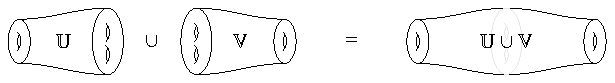
\includegraphics[width=0.62\textwidth]{figures/Fig_052_PDF127_Book115.pdf}
  \caption{沿共同边界粘合两个区域（原书 p.115）}
  \label{fig:cobordism-gluing}
\end{figure}

配边范畴\index{peibianfanchou@配边范畴|hyperpage} $\mathrm{Cob}_n$ 的对象是定向的 $(n-1)$ 维流形，态射是带边界的定向 $n$ 维流形。态射 $U$ 的边界分成两个不交部分 $B_i$ 与 $B_o$：后者继承 $U$ 的定向，前者取相反定向。这样，$U$ 就被视为从 $B_i$ 到 $B_o$ 的态射。两个态射通过公共边界粘合而复合。

根据流形带有的结构（拓扑、光滑、Riemann 度量等），配边范畴有不同版本。量子场论可以看成从适当配边范畴到 Hilbert 空间范畴的函子，并满足一些附加性质。最重要的附加条件是函子必须是幺半的：它把边界分量的不交并映到向量空间的张量积。若配边范畴是拓扑范畴，我们就称之为拓扑量子场论（TQFT）。更多信息可参见\bookcite{246,18}。

\begin{note}\label{note:qft-cobordism}
\textbf{观察 5.11.} 量子场论研究配边范畴的幺半表示。
\end{note}

\subsection{闭弦}
这一观点也适用于弦理论。闭弦是嵌入靶流形中的圆 $\sigma\colon S^1\to X$。弦随时间运动时，会在 $X$ 中扫出一个圆柱。弦还可能出现更复杂的行为，例如产生或消失，或者两条弦融合。这些动力学可以对应到如下配边：
\begin{figure}[H]
  \centering
  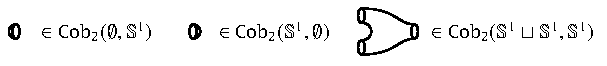
\includegraphics[width=0.74\textwidth]{figures/Fig_053_PDF128_Book116.pdf}
  \caption{闭弦的产生、湮灭与融合（原书 p.116）}
  \label{fig:closed-string-cobordisms}
\end{figure}

为了构造弦的量子理论，我们给每组弦指派一个 Hilbert 空间，并让世界面作为这些空间之间的线性映射；映射系数由适当的作用量原理给出。这自然可以看成二维配边范畴的幺半表示。拓扑弦理论给出从 $\mathrm{Cob}_2$ 到 $\mathrm{Hilb}$（或 $\mathrm{Vect}(k)$）的函子。由于每个拓扑曲面都可以由裤子曲面、圆帽和圆杯拼成，该函子由 $V=F(S^1)$ 和上述三种操作的像决定：单位映射 $k\to V$、迹映射 $V\to k$ 和乘法 $V\otimes V\to V$。这三项数据使 $V$ 成为一个 Frobenius 代数\index{frobeniusdaishu@Frobenius 代数|hyperpage}\bookcite{8}。

\begin{note}\label{note:tqft-frobenius}
\textbf{观察 5.12.} 二维 TQFT 与 Frobenius 代数一一对应。
\end{note}

大多数弦理论并非拓扑理论，而是共形理论，也就是说还必须考虑世界面的复结构\bookcite{215}。相应的共形配边范畴 $\mathrm{CFT}$ 对每个圆的 $n$ 元组有一个对象 $n$；$\mathrm{CFT}(n,m)$ 是带有 $n+m$ 个边界分量的 Riemann 曲面的模空间，并附有与各边界的 $S^1$ 的识别（标架）。该空间按曲面亏格分解为不交并：
\[
  \mathrm{CFT}(n,m):=\coprod_g\mathcal N_{g,n+m}.
\]
给定一个弦理论后，可以尝试计算相应函子 $\mathrm{CFT}\to\mathrm{Hilb}$。此函子把对象 $n$ 映到 Hilbert 空间 $H^{\otimes n}$，其中 $H$ 描述单条弦的所有状态。若在 $\mathrm{CFT}(n,m)$ 中固定一个点（即固定一个曲面 $\Sigma$），路径积分形式会给出映射 $H^{\otimes n}\to H^{\otimes m}$，它由对曲面 $\Sigma$ 上所有可能场构型积分得到。

不仅如此，我们还可以把积分扩展到 $\mathrm{CFT}(n,m)$ 的某个子空间中的所有曲面构型，而不只取一个点。这样，奇异链复形中的每条链都会给出一个映射 $H^{\otimes n}\to H^{\otimes m}$。为使这一想法精确化，定义范畴 $\mathrm{HCFT}^\bullet$：其对象为 $n\in\mathbb N$，而 $\mathrm{HCFT}^\bullet(n,m)$ 是适当的复形，用于计算 $\mathrm{CFT}(n,m)$ 的同调。从这一角度看，路径积分形式可解释为幺半 dg-函子
$F\colon\mathrm{HCFT}^\bullet\to\mathrm{dgVect}^\bullet$。这称为拓扑共形场论\index{tuopugongxingchanglun@拓扑共形场论|hyperpage}\bookcite{90,58,214}。

\begin{example}[A 模型与 Gromov--Witten 不变量]
在 A 模型中，这一思想与 Gromov--Witten 不变量\index{gromovwittenbubianliang@Gromov–Witten 不变量|hyperpage}\bookcite{85}密切相关。设 $X$ 是光滑射影簇，固定 $n,g\in\mathbb N$ 和一个 $2$-循环 $\beta\in H_2(X,\mathbb Z)$。给定 $n$ 个上同调类 $\psi_1,\ldots,\psi_n\in H^\bullet(X,\mathbb Q)$，可以定义 Gromov--Witten 不变量
\[
  GW^X_{\beta,g,n}(\psi_1,\ldots,\psi_n)
  \in H^\bullet(\mathcal M_{g,n},\mathbb Q).
\]
它是 $\mathcal M_{g,n}$ 上的上同调环元素；$\mathcal M_{g,n}$ 是亏格为 $g$、带有 $n$ 个标记点的 Riemann 曲面模空间的紧化（此处是标记点而非边界圆，因此没有标架）。直观上，这些不变量应当计数这样的全纯映射 $\sigma\colon\Sigma\to X$：曲面 $\Sigma$ 的亏格为 $g$，有 $n$ 个标记点，$\sigma(\Sigma)$ 的同调类为 $\beta$，且这些标记点落在与 $\psi_i$ 对偶的同调类上。

下面简述如何把这些数据转化为 $\mathrm{HCFT}^\bullet$ 的表示。取 $H_2(X,\mathbb Z)$ 的一组基 $\beta_1,\ldots,\beta_k$，并令 $K=\mathbb C((t_1,\ldots,t_k))$。若 $\beta=b_1\beta_1+\cdots+b_k\beta_k$，则置 $t^\beta=t_1^{b_1}\cdots t_k^{b_k}$。考察向量空间 $V=H^\bullet(X,K)$。因为 $X$ 光滑且紧致，$V$ 带有双线性配对 $\langle-,-\rangle\colon V\times V\to K$，由此可将 $V$ 与其 $K$-对偶空间识别，并将任意线性映射 $f\colon V^{\otimes_K n}\to V^{\otimes_K m}$ 看作映射 $f\colon V^{\otimes_K(n+m)}\to K$。

固定这些约定后，可以把 Gromov--Witten 不变量转化为 $\mathrm{HCFT}^\bullet$ 的表示。令 $GW^X(n)=V^{\otimes_K n}$；对任意 $\eta\in\mathrm{HCFT}^\bullet(n,m)$，令 $GW^X(\eta)$ 对应于映射
\[
  V^{\otimes_K(n+m)}\to K:\quad
  \psi_1\otimes\cdots\otimes\psi_{n+m}\longmapsto
  \sum_\beta t^\beta\int_\eta
  GW^X_{\beta,g,n+m}(\psi_1,\ldots,\psi_{n+m}).
\]
换言之，映射的系数是对循环 $\eta$ 积分后、再加权求和得到的 Gromov--Witten 不变量，并把 $\eta$ 重新解释为 $\mathcal M_{g,n+m}$ 中的循环。更多细节可参见\bookcite{58}。反过来，从拓扑共形场论出发，也可以计算出某些类似 Gromov--Witten 不变量的数值不变量\bookcite{61,50}。
\end{example}

\begin{note}\label{note:closed-strings-cft}
\textbf{观察 5.14.} 闭弦理论给出 $\mathrm{CFT}$ 或 $\mathrm{HCFT}^\bullet$ 的表示。
\end{note}

\subsection{开弦}
闭弦是嵌入时空的圆，但我们也可以考虑开弦，即嵌入的线段。为了描述开弦的动力学，还必须研究其端点处发生的事情。一般而言，端点被限制在靶空间 $X$ 的某些子流形上，而端点处的场取值在这些子流形上的某些丛中。

这些带有丛的子流形应被视为自身也具有动力学的对象。在物理学中，它们称为膜\index{mo@膜|hyperpage}（brane）；依弦理论模型不同，膜有不同类型。与闭弦理论一样，可以把它们纳入范畴形式体系\bookcite{16}：
\begin{itemize}
  \item 膜是范畴的对象；
  \item 膜之间的交点给出它们之间的态射；
  \item 乘法由弦在这些交点之间运动的方式决定。
\end{itemize}
对固定靶空间 $(X,J,\omega)$，我们得到两个由膜构成的 $A_\infty$ 范畴，一个对应 A 模型，一个对应 B 模型。
\begin{itemize}
  \item A 模型使用辛几何，膜是拉格朗日子流形。它们是满足 $\omega|_{TL}=0$ 的极大子流形 $L\subset X$。对应范畴称为 Fukaya 范畴，其数学定义将在第六章给出。
  \item B 模型中的子流形是复子流形。进一步考虑可知，还必须允许在这些子流形上带有某些丛。这便引出相干层导出范畴的概念，其数学定义将在第七章给出。
\end{itemize}

这些膜范畴与前面讨论的共形场论有何关系？从物理角度看，把开弦接在一起形成闭弦是很自然的，因此原则上可以由开弦版本构造闭弦理论。Costello 在文献\bookcite{58}中证明了这一点。对每个对象集 $\Lambda$，他构造了三个 dg-范畴：$\mathcal O^\bullet_\Lambda$ 描述端点落在 $\Lambda$ 中对象上的开弦；混合版本 $\mathcal{OC}^\bullet_\Lambda$ 同时包含开弦和闭弦；子范畴 $\mathcal C^\bullet$ 则只描述闭弦。最后一个范畴与 $\mathrm{HCFT}^\bullet$ 拟等价，且不依赖 $\Lambda$。它们之间的关系为
\[
  \mathcal O^\bullet_\Lambda\subset
  \mathcal{OC}^\bullet_\Lambda\supset\mathcal C^\bullet.
\]
若有 $\mathcal O^\bullet_\Lambda$ 的一个表示，就可以将其延拓为 $\mathcal{OC}^\bullet_\Lambda$ 的表示，再限制为 $\mathcal C^\bullet$ 的表示。后者可解释为一个上同调共形场论。Costello 还证明，给出 $\mathcal O^\bullet_\Lambda$ 的一个表示，等价于构造一个以 $\Lambda$ 为对象集的（循环）$A_\infty$ 范畴。此外还可证明，导出等价的 $A_\infty$ 范畴会给出等价的 $\mathcal C^\bullet$ 表示。

\begin{note}\label{note:open-string-ainfty}
\textbf{观察 5.15.} 开弦理论由（循环）$A_\infty$ 范畴决定，而导出等价的 $A_\infty$ 范畴给出等价的闭弦理论。
\end{note}

\section{何谓镜像对称？}
在 20 世纪 80 年代和 90 年代，物理学家注意到：某个 Kähler 流形 $X$ 上 A 模型的一些计算，与另一个流形 $X^\vee$ 上 B 模型的计算相吻合。因此他们猜想，每个 A 模型都应当有一个定义在另一流形上的 B 模型，使二者在物理上等价。这一新现象称为镜像对称，而一对流形 $(X,X^\vee)$ 称为镜像对。这个名称源自一种数值不变量：镜像对的 Hodge 菱形\index{hodgelingxing@Hodge 菱形|hyperpage}互为镜像。下图展示五次三维簇及其镜像的 Hodge 菱形：

\takeaway{镜像对称最初表现为一对流形 $(X,X^\vee)$ 上 A/B 模型计算相符、Hodge 菱形互为镜像；Kontsevich 把它提升为同调镜像对称：$D^\pi\mathrm{Fuk}(X)\cong D^\pi\mathrm{Coh}(X^\vee)$ 的 $A_\infty$ 拟等价，其数值不变量对应 Gromov--Witten 不变量与周期。}
\begin{figure}[H]
  \centering
  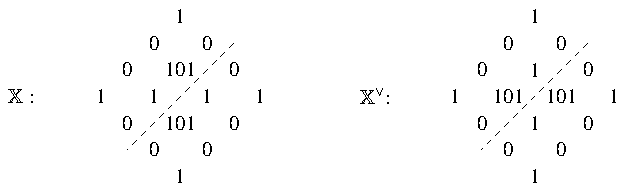
\includegraphics[width=0.88\textwidth]{figures/Fig_054_PDF131_Book119.pdf}
  \caption{五次三维簇及其镜像的 Hodge 菱形（原书 p.119）}
  \label{fig:quintic-hodge-diamonds}
\end{figure}

从数学角度看，这意味着辛几何中的某些问题可以通过在另一流形上做复几何来回答，反之亦然。起初，大多数数学家觉得这个想法近乎荒谬；但当物理学家 Candelas、de la Ossa、Green 和 Parkes\bookcite{51}用它来计数五次三维簇上的曲线时，数学家开始重视它。这些数目可以用 Gromov--Witten 不变量严格定义，但一直很难确定\bookcite{75}；借助镜像对称，Candelas 等人把它们联系到镜像流形上的某些积分（称为周期），并求得它们的生成级数。

人们提出了许多形式化镜像对称的方法。起初，这些表述都采用经典几何框架，使用微分几何、辛几何、复几何和枚举几何中的标准工具\bookcite{92,158}。1994 年，Kontsevich\bookcite{141}提出从范畴论角度考察镜像对称，由此引出了同调镜像对称\index{tongdiaojingxiangduichen@同调镜像对称|hyperpage}的思想。

其核心思想是：镜像对称应当体现为两个 $A_\infty$ 范畴之间的导出等价。一个范畴对应 A 模型，称为 Fukaya 范畴；另一个对应 B 模型，是相干层的导出范畴。其理由是，既然超弦理论可以看成某个 $A_\infty$ 范畴的表示，那么导出等价的 $A_\infty$ 范畴就会给出相同的物理学。数学上，范畴等价又意味着这些范畴的某些数值不变量相同；将这些不变量分别放回辛几何和代数几何的背景中，便可恢复较经典的镜像对称陈述：
% [Tutor Note: 这里 $D^\pi$ 表示分裂导出范畴；同调镜像对称断言的是 $A_\infty$ 拟等价，而不只是三角等价。物理上“导出等价给出相同物理”依赖开闭弦对应：开弦范畴决定闭弦理论（Costello 定理）；数学上还需为 $\mathrm{Coh}(X^\vee)$ 选好增强三角结构，才能谈论 $A_\infty$ 范畴。]
\begin{figure}[H]
  \centering
  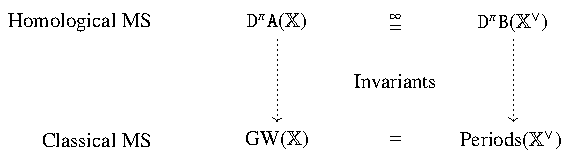
\includegraphics[width=0.68\textwidth]{figures/Fig_055_PDF132_Book120.pdf}
  \caption{同调镜像对称与经典镜像对称之间的关系（原书 p.120）}
  \label{fig:hms-classical-mirror}
\end{figure}

最初，镜像对称只针对一类特殊的 Kähler 流形——紧致 Calabi--Yau 流形提出。后来人们逐渐认识到，这一原理还可推广到其他几何背景：相关空间可以不是 Calabi--Yau\bookcite{5,139,49}，可以非紧\bookcite{1}、非光滑\bookcite{199}，甚至可以非交换\bookcite{11}。为了处理这些新空间，人们构造了 A 模型和 B 模型的若干推广。

接下来的两章将讨论这些 $A_\infty$ 范畴的构造。我们先研究 A 模型及 Fukaya 范畴的不同版本；对 B 模型，我们将定义相干层导出范畴这一 $A_\infty$ 范畴，并考察矩阵分解范畴。本部分最后一章将给出 A 模型与 B 模型等价的若干例子，以展示同调镜像对称这一现象。我们还将讨论如何借助环面几何和热带几何的思想寻找镜像对 $(X,X^\vee)$，并简要勾勒这与该领域两条重要研究方向——SYZ 猜想\bookcite{237}和 Gross--Siebert 纲领\bookcite{104,105}——之间的联系。

\section{练习}
\begin{exercise}\label{exer:physics-free-particle}
令 $M=\mathbb R^2$，并设 $\gamma\colon[0,1]\to M$ 是一条路径。自由运动粒子的经典作用量为 $S(\gamma)=\int_0^1\dot\gamma^2(t)\,dt$。证明：在 $X(x_0\to x_1)$ 中使作用量取极小值的曲线 $\gamma$，以恒定速度沿从 $x_0$ 到 $x_1$ 的直线运动。
\end{exercise}

\begin{exercise}\label{exer:discrete-path-integral}
令 $M=\mathbb R^2$，并令 $I_3=\{0,\frac12,1\}$。离散路径空间为
\[
  X_3(x_0\to x_1):=\{\gamma\colon I_3\to M\mid
  \gamma(0)=x_0,\ \gamma(1)=x_1\}=M,
\]
其上的作用量为
\[
  S(\gamma)=r\left((x_1-\gamma(\tfrac12))^2+
                     (\gamma(\tfrac12)-x_0)^2\right),
\]
其中 $r$ 为常数。证明：路径积分中 $\gamma(\frac12)$ 的期望值为 $(x_0+x_1)/2$。可以假设 $r\in\mathbb C$ 的选取使相关积分收敛。
\end{exercise}

\begin{exercise}\label{exer:loop-rotation-observable}
令 $M=\mathbb C$，并考察闭曲线空间
\[
  X=\{\gamma\colon[0,1]\to M\mid\gamma(0)=\gamma(1)\}.
\]
对与曲线起点旋转对应的向量场 $Q$，都有一参数对称性
\[
  \exp(\epsilon Q)(\gamma)(t)=\gamma(t+\epsilon\bmod1),
\]
它对应于改变曲线的起点。令可观测量 $X_u:=\gamma(u)$，即把曲线 $\gamma$ 映到其在时刻 $u$ 的位置。求 $d_QX_u$。
\end{exercise}

\begin{exercise}\label{exer:lie-algebra-cohomology}
设 Lie 代数 $\mathfrak g=\mathbb Rg_1+\cdots+\mathbb Rg_k$ 作用于空间 $X$。考虑张量积
\[
  K^\bullet:=C^\infty(X)\otimes\Lambda^\bullet(\mathfrak g)
  =C^\infty(X)\otimes
  \frac{\mathbb C\langle g_1,\ldots,g_k\rangle}
  {\langle g_ig_j+g_jg_i\mid1\le i,j\le k\rangle},
\]
并定义微分
\[
  d(\phi g_{i_1}\cdots g_{i_r})=
  \sum_j(g_j\cdot\phi)\,g_j\wedge g_{i_1}\wedge\cdots\wedge g_{i_r}.
\]
证明这是一个复形，并且
\[
  H^0(K)=\{f\in C^\infty(X)\mid
     \forall g\in\mathfrak g,\ g\cdot f=0\}.
\]
再证明：若 $\mathfrak g$ 在 $X$ 上的作用是自由的（即每一点处与 $g_i$ 对应的向量场线性无关），则 $H^1(K)=0$；事实上，所有更高次上同调也都为零。
\end{exercise}

\begin{exercise}\label{exer:susy-invariant-action}
证明作用量
\[
  S=\frac12V(x)^2-\psi_+\psi_-\frac{d}{dx}V(x)
\]
在超对称变换 $Q_\pm$ 下确实不变。
\end{exercise}

\begin{exercise}\label{exer:susy-auxiliary-field}
考虑一个包含两个玻色场 $x,H$ 和两个费米场 $\psi_+,\psi_-$ 的系统。证明作用量
\[
  S=\frac12H^2+iHV(x)-\psi_+\psi_-\frac{d}{dx}V(x)
\]
具有如下超对称性：
\[
  \delta x=\psi_++\psi_-,\qquad
  \delta\psi_\pm=\pm iH,\qquad \delta H=0,
\]
并证明 $\delta^2=0$，且存在表达式 $F$ 使 $S=\delta F$。
\end{exercise}

\begin{exercise}\label{exer:oriented-riemann-kaehler}
证明：每个二维可定向 Riemann 流形都可以看成 Kähler 流形，其中复结构 $J$ 对应于逆时针旋转 $90^\circ$。
\end{exercise}

\begin{exercise}\label{exer:cobordism-one-category}
拓扑配边范畴 $\mathrm{Cob}_1$ 的对象是带符号点集，即每个点都附有 $+$ 或 $-$ 号的有限点集。态射由若干条定向开曲线构成：曲线从 $S_1$ 的正点或 $S_2$ 的负点出发，到达 $S_2$ 的正点或 $S_1$ 的负点；此外还可带有若干条闭曲线。若两个态射之间存在保持端点的同胚，就认为它们相同。
\begin{enumerate}[label=(\roman*)]
  \item 令 $S=\varnothing$。证明 $\mathrm{Cob}_1(S,S)$ 在复合运算下同构于 $(\mathbb N,+)$。
  \item 令 $S=\{p_1^+,\ldots,p_k^+\}$。证明 $\mathrm{Cob}_1(S,S)$ 在复合运算下同构于 $\mathbb N\times S_k$。
  \item 令 $S=\{p^+,q^-\}$。描述半群 $\mathrm{Cob}_1(S,S)$。
\end{enumerate}
\end{exercise}

\begin{exercise}\label{exer:monoidal-cobordism-functor}
函子 $F\colon\mathrm{Cob}_1\to\mathrm{vect}(k)$ 称为幺半函子，若它把带点集的不交并自然地映为张量积：
\[
  F(S_1\sqcup S_2)\cong F(S_1)\otimes F(S_2).
\]
类似地，它也把曲线的不交并映为映射的张量积。精确定义见\bookcite{246}。
\begin{enumerate}[label=(\roman*)]
  \item 证明 $F$ 由下列两个基本配边的像决定：
  \begin{figure}[H]
    \centering
    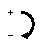
\includegraphics[width=0.15\textwidth]{figures/Fig_056_PDF134_Book122.pdf}\qquad
    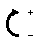
\includegraphics[width=0.15\textwidth]{figures/Fig_057_PDF134_Book122.pdf}
    \caption{一维配边范畴的基本生成态射（原书 p.122）}
    \label{fig:cobordism-one-generators}
  \end{figure}
  \item 证明下图的像给出 $V_+:=F(+)$ 与 $V_-:=F(-)$ 之间的非退化配对。由此推出：每个维数 $n\in\mathbb N$ 恰好对应一个一维 TQFT。
  \begin{figure}[H]
    \centering
    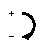
\includegraphics[width=0.18\textwidth]{figures/Fig_058_PDF135_Book123.pdf}
    \caption{诱导配对的配边（原书 p.123）}
    \label{fig:cobordism-pairing}
  \end{figure}
  \item 在无定向配边范畴中，对象只是点集，态射是这些点之间的无定向曲线。描述该范畴及其幺半表示。
\end{enumerate}
\end{exercise}

\begin{exercise}\label{exer:two-dimensional-tqft-frobenius}
设 $F$ 是一个二维 TQFT。证明：相应 Frobenius 代数中的乘法是结合且交换的。此外，证明配对 $(a,b)\mapsto\operatorname{Tr}(a\cdot b)$ 非退化。
\end{exercise}

\chapterreview{%
\textbf{全章地位。}这是全书唯一的物理章，任务不是证明而是建词典：把路径积分、对称性、超对称、超弦这些物理语言逐条翻译成上同调与范畴。第 4 章已在例子里见到 A/B 二重性，第 6、7 章要给出严格构造，本章负责说明这些构造为何值得做。

\textbf{知识脉络。}先立最小作用量原理：物理演化是作用量 $S$ 在路径空间 $X$ 上的临界点；量子化则把可观测量写成 $\int Fe^{iS/\hbar}[d\gamma]$，$\hbar\to0$ 时只有经典解存活。接着把对称性代数化：群作用保持 $S$ 与测度，无穷小生成元给出导子 $d_Q$，物理上的不可区分性把可观测量压成 $\ker d_Q/\operatorname{im}d_Q$；若 $S=d_QV$，期望值与 $\hbar$ 无关，这正是局域化的雏形。然后加入费米场得到超对称，在零维模型上算出 $Z_{\mathrm{SUSY}}$ 只是经典解的带符号计数。把同一套超对称搬到二维世界面，就得到 $d=2,N=(2,2)$ 理论；保留不同的子代数分别给出只依赖辛结构的 A 模型与只依赖复结构的 B 模型。最后用函子重述：粒子是 $\mathrm{Part}$ 的表示，量子场论是配边范畴到 $\mathrm{Hilb}$ 的幺半函子，二维 TQFT 等价于 Frobenius 代数，开弦由（循环）$A_\infty$ 范畴描述并决定闭弦理论。

\textbf{核心结论。}（1）路径积分的配分函数与期望值为 $Z=\int_Xe^{iS/\hbar}[d\gamma]$、$\langle F\rangle=\int_XFe^{iS/\hbar}[d\gamma]$，半经典极限只留下满足 $\delta S=0$ 的经典解。（2）对称性给出上同调：可观测量取在 $\ker d_Q/\operatorname{im}d_Q$ 中；当 $S=d_QV$ 且 $d_QF=0$ 时 $\langle F\rangle$ 与 $\hbar$ 无关，于是可把积分约化到经典解上。（3）A 模型的配分函数只依赖 $(X,\omega)$，其数值不变量是计数全纯映射的 Gromov--Witten 不变量；B 模型只依赖 $(X,J)$，局部可观测量是 Dolbeault 上同调。（4）二维 TQFT 与 Frobenius 代数一一对应；开弦范畴决定闭弦的共形场论，导出等价的 $A_\infty$ 范畴给出相同的物理。（5）同调镜像对称的表述：$D^\pi\mathrm{Fuk}(X)$ 与 $D^\pi\mathrm{Coh}(X^\vee)$ 之间存在 $A_\infty$ 拟等价，其数值影子是 Gromov--Witten 不变量与周期。

\textbf{辨析与提醒。}其一，说 A 模型“只依赖辛结构”，是就计数与面积而言；全纯性本身当然用到了复结构 $J$，$J$ 只用于写方程，且在形变下不改变计数。这个区别最容易被误读成“A 模型不需要复结构”。其二，路径积分测度 $[d\gamma]$ 并不存在，本章明言“假定这样的测度存在”；真正把上述形式严格化的是局部化与 Gromov--Witten 理论，读者不宜把零维模型的计算当作一般证明。其三，开弦决定闭弦（Costello）是物理输入，方向不能反过来用；而 $\hbar\to0$ 的论证依赖 $d_Q$ 在测度上无反常、边界项可忽略，正文只用一句“乐于研究”带过。

\textbf{评注。}本章的取舍很清楚：只在一个零维超对称模型上把 Grassmann 积分、Berezin 规则与带符号计数完整算一遍，其余全部以作用量与观察的形式给出。对数学读者，这足以建立“上同调即物理可区分性”的直觉；对物理读者则显得过于简略。真正的价值在于那条层级链：经典临界点 $\to$ 路径积分 $\to$ 对称性上同调 $\to$ 超对称 $\to$ 弦 $\to$ 范畴，每一步都为下一步提供对象。作者有意不展开镜像对称的枚举几何细节（曲线计数只作引子），把技术留给后续章节，这与全书“先给图景、再补定义”的策略一致。读本章不必纠缠符号约定，抓住两件事即可：$S=d_QV$ 导致局域化；A/B 模型的差别只在于保留哪一个超对称子代数。}
